% !TeX program = lualatex -synctex=1 -interaction=nonstopmode --shell-escape %.tex

\documentclass[_Banking_p2.tex]{subfiles}
\begin{document}

\setbeamercovered{invisible}
\subsection{Нормативные документы}
\begin{frame}[allowframebreaks]{Ипотечные операции банков}{Нормативные документы}
  \begin{thebibliography}{10}
  
  \beamertemplatearticlebibitems

    \bibitem{bb2}
Федеральный закон от 11.11.2003 N 152-ФЗ (ред. от 01.07.2017) "Об ипотечных ценных бумагах"

    \bibitem{bb2}
Федеральный закон от 16.07.1998 N 102-ФЗ (ред. от 01.07.2017) "Об ипотеке (залоге недвижимости)"

    \bibitem{bb2}
Постановление Правительства РФ от 26.08.1996 N 1010 "Об Агентстве по ипотечному жилищному кредитованию"

\pagebreak

    \bibitem{bb2}
Инструкция Банка России от 14.04.2015 N 162-И (ред. от 11.05.2017) "О требованиях к составу и содержанию документов, представляемых в Банк России для регистрации правил доверительного управления ипотечным покрытием, а также изменений и дополнений, вносимых в них" 

    \bibitem{bb2}
Инструкция Банка России от 31.03.2004 N 112-И (ред. от 14.11.2012) "Об обязательных нормативах кредитных организаций, осуществляющих эмиссию облигаций с ипотечным покрытием"

\pagebreak

    \bibitem{bb2}
Приказ ФСФР РФ от 01.11.2005 N 05-59/пз-н (ред. от 21.01.2011) "Об утверждении Положения о порядке определения размера ипотечного покрытия" (Зарегистрировано в Минюсте РФ 13.12.2005 N 7265)

    \bibitem{bb2}
Постановление Правительства РФ от 15.10.2004 N 562 (ред. от 01.06.2010) "Об утверждении Типовых правил доверительного управления ипотечным покрытием"

\pagebreak

    \bibitem{bb2}
Постановление Правительства РФ от 13.03.2015 N 220 (ред. от 17.04.2017) "Об утверждении Правил предоставления субсидий из федерального бюджета российским кредитным организациям и акционерному обществу "Агентство ипотечного жилищного кредитования" на возмещение недополученных доходов по выданным (приобретенным) жилищным (ипотечным) кредитам (займам)"

\pagebreak

    \bibitem{bb2}
Указание Банка России от 03.04.2015 N 3610-У "Об отражении в бухгалтерском учете расходов от реструктуризации ипотечных жилищных ссуд, предоставленных физическим лицам в иностранной валюте до 1 января 2015 года"

    \bibitem{bb2}
Приказ Минтруда России от 19.03.2015 N 171н "Об утверждении профессионального стандарта "Специалист по ипотечному кредитованию"

    \bibitem{bb2}
Приказ Министра обороны РФ от 24.04.2017 N 245 "Об утверждении Порядка реализации накопительно-ипотечной системы жилищного обеспечения военнослужащих в Вооруженных Силах Российской Федерации"

    \bibitem{bb2}
Постановление Правительства РФ от 10.03.2009 N 209 "О предоставлении межбюджетных трансфертов бюджету Пенсионного фонда Российской Федерации на погашение за счет средств материнского (семейного) капитала основного долга и уплату процентов по кредитам или займам на приобретение (строительство) жилого помещения, в том числе ипотечным, предоставленным гражданам по кредитному договору (договору зай...

\end{thebibliography}
\end{frame}

\subsection{Секьюритизация ипотеки}
\begin{frame} {Секьюритизация ипотеки}

\begin{block}{Секьюритизация от англ. securities – ценные бумаги}
\quad
- это процесс, в ходе которого осуществляется выпуск ценных бумаг, обеспеченных активами.
\end{block}

Сущность механизма секъюритизации заключается в процедуре преобразования долговых обязательств, связанных с рефинансированием, в бумаги, обладающие приемлемым обеспечением и сравнительно высокой ликвидностью.

\end{frame}

\begin{frame}{Процедурная сторона секьюритизации }
Кредитные организации, осуществляющие ипотечное кредитование, выпускают обеспеченные ценные бумаги. 

Ипотечные инвесторы продают долговые обязательства ипотечному агенту  - специализированной коммерческой организации, которая в конечном итоге осуществляет эмиссию обеспеченных ценных бумаг, поскольку обладает правом осуществлять эмиссию облигаций с ипотечным покрытием.
\end{frame}


\begin{frame}
\begin{block}{Ипотечные облигации,\\ англ. Mortgage-Backed Securities (MBS)}
\quad
- это ценные бумаги, выпущенные в процессе секьюритизации и обеспеченные ипотечными активами.
\end{block}

\begin{block}{Обеспеченные активами облигации,\\ англ. Asset Backed Securities (ABS)}
\quad
- это ценные бумаги, выпущенные в процессе секьюритизации обязательств по другим видам кредитов, не связанных с ипотекой.
\end{block}
\end{frame}

\begin{frame} {Ипотечные ценные бумаги в США}
\begin{itemize}[<	+->]

\item
ценные бумаги, выпускаемые агентствами с поддержкой Правительства США, англ. Government-Sponsored Enterprises, под гарантию агентств, известные как агентские ипотечные ценные бумаги, англ. agency MBS;

\item
ценные бумаги, выпускаемые частными институтами, известные как частные ипотечные ценные бумаги, англ. non-agency MBS.
\end{itemize}
\end{frame}

\begin{frame}{Квазиправительственные ипотечные агентства в США}
\begin{itemize}[<+->]
\item
Государственная национальная ипотечная ассоциация Ginnie Мае.
\item
Федеральная ипотечная корпорация жилищного кредитования Freddie Мае.
\item
Федеральная национальная ипотечная ассоциация Fannie Мае.
\end{itemize}
\end{frame}

\begin{frame}[shrink=20]
\begin{figure}
	\center
	\begin{overprint}
		\forloop{slideno}{1}{\value{slideno} < 8}{%
			\only<\value{slideno}>{
				\includegraphics[page=\value{slideno},
				scale=1
				% trim={<left> <lower> <right> <upper>}				
				,trim={.5cm 4.5cm 1cm 0cm},clip]
				{tikz/mortgage_scheme}}}
	\end{overprint}
	\vspace*{-1.5em}
	\caption{Схема выпуска ценных бумаг,\\ обеспеченных активами, в США}
\end{figure}
\only<2>{
	1) заемщики заключают с банком кредитный договор на покупку недвижимости под залог;
}

\only<3>{
	2) организатор секьюритизации вместе с рейтинговым агентством, страховой компанией, риэлтерами, банком-гарантом создают траст; 
}

\only<4>{
	3) ипотечные кредиты размещаются банком при посредничестве организатора в специально созданном трасте;
}

\only<5>{
	4) эмитенты выпускают ипотечные облигации, обеспеченные активами траста и размещают их при посредничестве банков андеррайтеров среди инвесторов;
}

\only<6>{
	5) деньги инвесторов, через посредников поступают банку-кредитору, что позволяет ему сразу вернуть средства, вложенные в кредитование;
}

\only<7>{
	6) выплаты заемщиков по ипотечным кредитам поступают держателям облигаций, за вычетом комиссионных, взимаемых посредниками.
}
\end{frame}

\begin{frame}{Характеристики ипотечных ценных бумаг}
\begin{itemize}[<	+->]
\item
платежи, выплачиваемые держателям ИЦБ, являются периодическими;

\item
платежи от пула активов обычно состоят из двух частей: процентной (плата за пользование кредитами) и амортизационной (погашение кредитов); 

\item
плановая амортизация представляет собой постепенное погашение баланса по кредиту таким образом, что к концу срока ипотечного кредита баланс оказывается погашен;
\end{itemize}
\end{frame}

\begin{frame}{Характеристики ипотечных ценных бумаг}
\begin{itemize}[<+->]
\item
досрочное погашение ИЦБ отражает тот факт, что в большинстве случаев заемщик по ипотечному кредиту имеет право на частичную или полную досрочную выплату кредита;

\item
уровень доходности ипотечных облигаций как долгового инструмента зависит от уровня риска невыплат, а также срока обращения. 
\end{itemize}
\end{frame}

\subsection{Рынок недвижимости}
\begin{frame}[shrink=15]{Тенденции рынка недвижимости в России}
\begin{figure}
\center
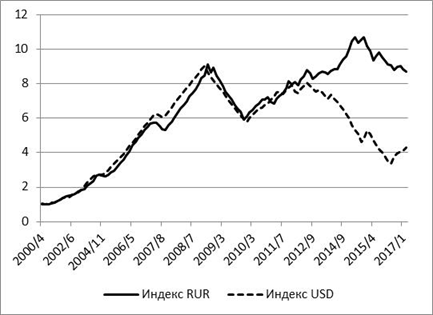
\includegraphics[scale=.8]{img/real_estate_price_index.png}
\caption{Индексы стоимости жилья в рублях и USD за квадратный метр за период с 01.04.2000 по 30.04.2017. \\
Источник: Информационное агентство "Индикаторы рынка недвижимости"  \url{http://www.irn.ru/},\\ дата обращения 5 мая 2017.}
\end{figure}
\end{frame}

\begin{frame}[shrink=15]{Тенденции рынка недвижимости в России}
\begin{figure}
\center
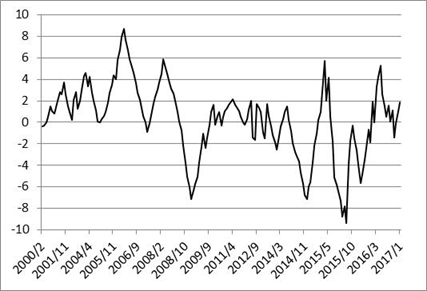
\includegraphics[scale=.8]{img/real_estate_price_expectations.png}
\caption{Индекс ожидания роста стоимости жилья \% в месяц за период с 1.02.2000 по 26.03.2017.\\
Источник: Информационное агентство "Индикаторы рынка недвижимости"  \url{http://www.irn.ru/},\\ дата обращения 5 мая 2017.}
\end{figure}
\end{frame}

\begin{frame}[shrink=15]{Тенденции рынка недвижимости в России}
\begin{figure}
\center
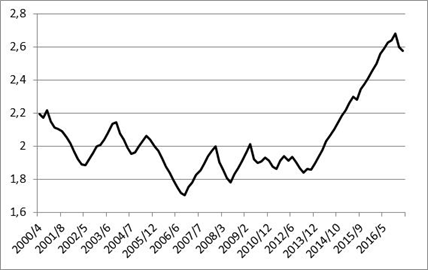
\includegraphics[scale=.8]{img/expencive_to_cheap_ratio.png}
\caption{Отношение стоимости "дорогого" жилья к "дешевому" (индекс расслоения) за период с 1.02.2000 по 26.03.2017. \\
Источник: Информационное агентство "Индикаторы рынка недвижимости"  \url{http://www.irn.ru/},\\ дата обращения 5 мая 2017.}
\end{figure}
\end{frame}


\subsection{Ценные бумаги}
\begin{frame}{Виды ипотечных ценных бумаг}
\begin{itemize}[<+->]
\item
закладная,
\item
облигация с ипотечным покрытием,
\item
ипотечный сертификат участия,

\item
жилищная облигация с ипотечным покрытием.
\end{itemize}
\end{frame}

\begin{frame}{}
\begin{block}{Закладная }
\quad
- это именная ценная бумага, удостоверяющая право своего законного владельца на получение исполнения по обязательству, обеспеченному залогом недвижимости. 

Назначение этой бумаги состоит в ускорении оборота заложенной недвижимости с целью расширения возможностей залогодержателя в скорейшем удовлетворении своих требований.
\end{block}
\end{frame}

\begin{frame}
\begin{itemize}[<+->]
\item
Передача прав по закладной залогодержателем осуществляется на основании цессии (уступки прав требований). 

\item
Наличие закладной не исключает необходимость заключения договора об ипотеке, условия которого должны предусматривать выдачу залогодержателю закладной. 

\item
Закладной предоставляется приоритет перед договором, так что, при несовпадении содержания контракта, положено руководствоваться содержанием закладной.
\end{itemize}
\end{frame}

\begin{frame}{}
\begin{block}{Облигация с ипотечным покрытием }
\quad
- это ценная бумага, исполнение обязательств по которой обеспечивается полностью или в части залогом ипотечного покрытия. 

Выпускается в документарной и бездокументарной формах. 
\end{block}
Главным образом на рынке обращаются жилищные облигации. При этом жилищные облигации не могут быть обеспечены залогом строящегося жилья.
\end{frame}

\begin{frame}
\begin{itemize}[<+->]
\item
Размер обязательств по всем находящимся в обращении облигациям с ипотечным покрытием должен составлять от 80\% до 100\% суммы ипотечного покрытия.
\item
Эмиссия облигаций с ипотечным покрытием может осуществляться исключительно кредитными организациями и ипотечными агентами, в роли которых выступают специализированные коммерческие организации (акционерные общества), основным видом деятельности которых является приобретение прав требований и выпуск ипотечных облигаций. 
\end{itemize}
\end{frame}

\begin{frame}{}
Норматив минимального соотношения размера ипотечного покрытия и объема эмиссии облигаций с ипотечным покрытием (H18):
\begin{align}
\text{Н18}=\frac{\text{ИП}}{\text{Обл}}\times 100\%,
\end{align}
где

ИП - размер ипотечного покрытия;

Обл - объем эмиссии облигаций с ипотечным покрытием (номинал + проценты).

\end{frame}

\begin{frame}{}
\begin{block}{Ипотечные сертификаты участия}
\quad
- это именная ценная бумага без номинальной стоимости, удостоверяющая долю её владельца в праве общей собственности на ипотечное покрытие, а также право требовать от выдавшего её лица надлежащего доверительного управления ипотечным покрытием и прочие права, предусмотренные законодательством и близкие к правам владельца инвестиционного пая. 
\end{block}
\end{frame}

\begin{frame}{}
Выдавать ипотечные сертификаты участия вправе только коммерческая организация (акционерное общество), имеющая лицензию на осуществление деятельности по управлению инвестиционными фондами, паевыми инвестиционными фондами и негосударственными пенсионными фондами. 
\end{frame}

\begin{frame}
Владение, хранение и учёт составляющих ипотечного покрытия осуществляются в соответствии с компетенцией управляющим и специализированным депозитарием. 
\end{frame}


\begin{frame}
Управляющий владеет, пользуется и распоряжается ипотечным покрытием в интересах владельцев ипотечных сертификатов участия. 

Депозитарий осуществляет контроль над деятельностью управляющего путем ведения реестра ипотечного покрытия.

\end{frame}

\begin{frame}
\begin{block}{Жилищная облигация с ипотечным покрытием }
\quad
– это облигация с ипотечным покрытием, в состав которого входят только права требования, обеспеченные залогом жилых помещений. 
\end{block}
\end{frame}


\subsection{Кредитоспособность}

\begin{frame}{Оценка кредитоспособности ипотечного заемщика}
1. Оценка способности заемщика своевременно погасить кредит на основе анализа его доходов и расходов.

2. Оценка кредитоспособности заемщика на основе анализа его кредитной истории, определяющей его готовность выполнять принимаемые финансовые обязательства.

3. Оценка достаточности наличных денежных средств (и источник формирования), которыми располагает потенциальный заемщик для выплаты первоначального взноса на покупку жилья и оплаты всех других необходимых расходов по совершаемым сделкам. 
\end{frame}

\begin{frame}{Оценка кредитоспособности ипотечного заемщика}
4. Проверка источников дохода заемщика. Заемщик должен представить документы о получении стабильного дохода за текущий отчетный период и за прошлый календарный год.

5. Анализ расходов заемщика: расходы по ипотечному кредиту, расчеты по содержанию объекта ипотеки, налоги на имущество, текущие расходы на содержание семьи, разовые ежегодные платежи или платежи с другой периодичностью в течение года (страхование и обслуживание автомобиля, отдых, образование детей и пр.).
\end{frame}
\begin{frame}{Источники денежных средств получения ипотечного кредита}
•	сбережения заемщика;

•	средства вырученные от продажи движимого или недвижимого имущества;

•	подарки от членов семьи;

•	подарки или гранты некоммерческих организаций не подлежащие возврату;
\end{frame}

\begin{frame}{Источники денежных средств получения ипотечного кредита}
•	подарки или гранты от работодателя, сделанные в рамках программы помощи сотрудникам, которая не должна быть возвращена или подлежит возврату после того, как будут исполнены обязательства по кредитному договору;

•	государственные жилищные субсидии.

Другое имущество заемщика (автомобиль, дача, ювелирные изделия, произведения искусства, антиквариат, другое ценное движимое и недвижимое имущество) не учитывается при оценке его кредитоспособности, но, оно может послужить дополнительной гарантией возврата кредита.
\end{frame}

\begin{frame}{Требования к ипотечному кредиту}
- покупка готового (построенного) жилья;

- коэффициент кредит/ залог , англ. Loan-to-value ratio, LTV  - от 70\% до 90\%;

- ставка процента по кредиту должна быть фиксированной;

- отдельный заемщик может получить только один ипотечный кредит;

- максимальный размер кредита для LTV равного от 71\% до 90\% не может превышать 8 млн рублей;
\end{frame}

\begin{frame}{Требования к ипотечному кредиту}
- срок кредита не может превышать 25 лет.

- если за последние два года имели место просрочки их выплат длительностью более 60 дней, максимальный размер ипотечного кредита, должен быть уменьшен на 25\%.

\end{frame}

\begin{frame}{Требования к заемщику}
- гражданство России;

- возраст - не менее 19 лет, а на момент окончания срока ипотечного кредита не должен превышать 65 лет;

- общая сумма ежегодных платежей по кредиту не должна быть больше 45\% годового дохода заемщика (коэффициент платеж / доход < 45\%);

- первоначальный взнос не менее 10\% стоимости предмета ипотеки.
\end{frame}


\begin{frame}{Способы проверки предоставленных заемщиком сведений}
-звонок в организацию / организации, где работает заемщик;

-выезд сотрудника банка на место работы сотрудника;

-приглашение заемщика в банк для личной встречи с сотрудником банка;

-выезд сотрудника банка на объект залога;

-обращение за дополнительной информацией о заемщике в соответствующее подразделение банка (службу безопасности и т.д.).
\end{frame}

\begin{frame}{Ипотека в России}{Агентство по ипотечному жилищному кредитованию}
\begin{itemize}[<	+->]
\item
Открытое акционерное общество «Агентство по ипотечному жилищному кредитованию» (Агентство, АИЖК) создано в 1997 году по решению Правительства РФ. 

\item
100\% акций АИЖК принадлежит государству в лице Федерального агентства по управлению государственным имуществом.
\end{itemize}
\end{frame}

\subsection{Ипотека в России}
\begin{frame}{Ипотека в России}{Агентство по ипотечному жилищному кредитованию}
\begin{itemize}[<	+->]

\item
Главная задача Агентства заключается в реализации государственной политики по повышению доступности жилья для населения России.


\item
Агентством создана система двухуровневого рефинансирования ипотечных жилищных кредитов (займов), участниками которой являются банки – первичные кредиторы, региональные операторы и сервисные агенты.
\end{itemize}
\end{frame}

\begin{frame}{Основные функции АИЖК}
\begin{itemize}[<+->]
\item
заключение долгосрочных договоров с партнерами на рефинансирование ипотечных жилищных кредитов и займов;
\item
внедрение различных финансовых инструментов и механизмов для повышения ликвидности и снижения рисков участников ипотечного рынка;
\item
привлечение финансовых ресурсов на ипотечный рынок путем выпуска и размещения на открытом рынке корпоративных облигаций и ипотечных ценных бумаг;
\end{itemize}
\end{frame}

\begin{frame}{Основные функции АИЖК}
\begin{itemize}[<+->]
\item
стандартизация порядка предоставления, оформления и обслуживания ипотечных жилищных кредитов и займов;
\item
предоставление технической и консультационной помощи участникам рынка ипотечного жилищного кредитования. 
\end{itemize}
\end{frame}

\begin{frame}[shrink=25]
% Table generated by Excel2LaTeX from sheet 'Лист1'
\begin{table}[htbp]
  \centering
  \caption{Рейтинг ипотечных банков-андеррайтеров в России, за первое полугодие 2016}
    \begin{tabular}{clrrrrr}
    \toprule
    \multirow{2}[4]{*}{№}     & \multirow{2}[4]{*}{Банк}  & \multicolumn{2}{c}{ОВК} & \multirow{2}[4]{*}{КВК} & \multirow{2}[4]{*}{КСС}   & \multirow{2}[4]{*}{ОИП} \\\cmidrule(lr){3-4}
          &       & ИКБ   & ИКВ   &       &       &  \\
    \midrule
    1     &  Сбербанк & 334   & н/д   & н/д   & 0     & 0 \\
    2     &  ВТБ 24 & 130   & 1417  & 781   & 28    & 226 \\
    3     &  Россельхозбанк & 31    & 198   & 149   & 0     & 0 \\
    4     &  Дельтакредит & 22    & 203   & 111   & 11    & 52 \\
    5     &  Газпромбанк & 20    & 348   & 168   & 2     & 22 \\
    \midrule
          & Всего по России & 593   & 2617  & 1418  & 48    & 366 \\
    \bottomrule
    \end{tabular}%
  \label{tab:addlabel}%
\end{table}%
{\scriptsize
Источник: расчеты автора по "Рэнкинг ведущих ипотечных банков по итогам 6 месяцев 2016 года" / Компания "Русипотека"; \url{http://rusipoteka.ru}, дата обращения 29 марта 2017.
Примечание: ОВК – Объем выданных кредитов, млрд руб; ИКБ – ипотечные кредиты на балансе банка; ИКВ – ипотечных кредитов выданные банком с начала деятельности; КВК – количество выданных ипотечных кредитов банком с начала деятельности, тыс. шт; КСС - количество сделок секьюритизации ипотечных кредитов с начала деятельности в качестве оригинатора и/или инициатора (балансовые и внебалансовые сделки), шт; ОИП - объем выпущенных облигаций с ипотечным покрытием с начала деятельности, включая балансовые сделки и сделки через Агента (номинал выпущенных бумаг), млрд руб.; н/д – нет данных.
\par}
\end{frame}

\begin{frame}{Пример операции секьюритизации ипотечного портфеля банка}
\begin{itemize}[<+->]
\item
Банк «Возрождение» завершил вторую сделку по секьюритизации ипотечного портфеля. Общий объем размещения составил 4 млрд рублей. 
\item
Облигации класса ``А'' на сумму 2,96 млрд рублей были размещены путем открытой подписки на Московской Бирже. Международное рейтинговое агентство Moody’s Investors Service присвоило им долгосрочный кредитный рейтинг на уровне Baa3. 
\end{itemize}
\end{frame}

\begin{frame}{Пример операции секьюритизации ипотечного портфеля банка}
\begin{itemize}[<+->]
\item
Облигации класса ``Б'' на сумму 1,04 млрд рублей путем закрытой подписки приобрел Банк ``Возрождение''. 
\item
Ценные бумаги были размещены по номинальной стоимости 1000 рублей, а эмитентом облигаций выступило Закрытое акционерное общество ``Ипотечный агент Возрождение 2''.
\end{itemize}
\end{frame}

\subsection{Контрольные вопросы}
\begin{frame}{Контрольные вопросы}
1. Понятие секьюритизации банковских ипотечных кредитов.

2. Ипотечные ценные бумаги используемые в США.

3. Обзор тенденций на рынке недвижимости в России.

4. Ипотечные ценные бумаги используемые в России.

5. Оценка кредитоспособности ипотечного заемщика.

6. Основные функции и показатели деятельности Агентства по ипотечному жилищному кредитованию.
\end{frame}

\setbeamercovered{transparent}
\end{document}
